\documentclass[dvipdfmx]{beamer}

\usepackage{beamerthemesplit}
\usepackage[]{graphicx}
\graphicspath{%
{./slide01-img/}%
{./text01-img/}%
}
% !TEX root = ./slide01-2.tex

\usepackage{listings}
\usepackage{hyperref}
\usepackage{pxjahyper}
\usepackage{color}

\setbeamertemplate{footline}[frame number]
\title{子どもIT未来塾 第1回}
\author{塾長 清水尚彦}

\def\quiz{1}

\begin{document}

\frame{
   \begin{center}
    \huge{子どもIT未来塾}\\

    \vspace{48pt}
	   \Large{第1回}\\
	   {\huge\bf ラズベリーパイの使い方・\\
	   \huge\bf 自己紹介ページを作ろう}\\
    \vspace{24pt}
    \large{塾長 清水尚彦}\\
    \vspace{10pt}
    \large{\the\year 年 6月24日}
  \end{center}
}



\begin{frame}[fragile]
	\frametitle{2時間目:ラズベリーパイになれよう(1) P.16-35~~~\raisebox{-3mm}{
\includegraphics[width=0.1\textwidth]{raspberry}}}
    \begin{description}
      \item[ラズベリーパイのそうさになれていこう]
    \end{description}
    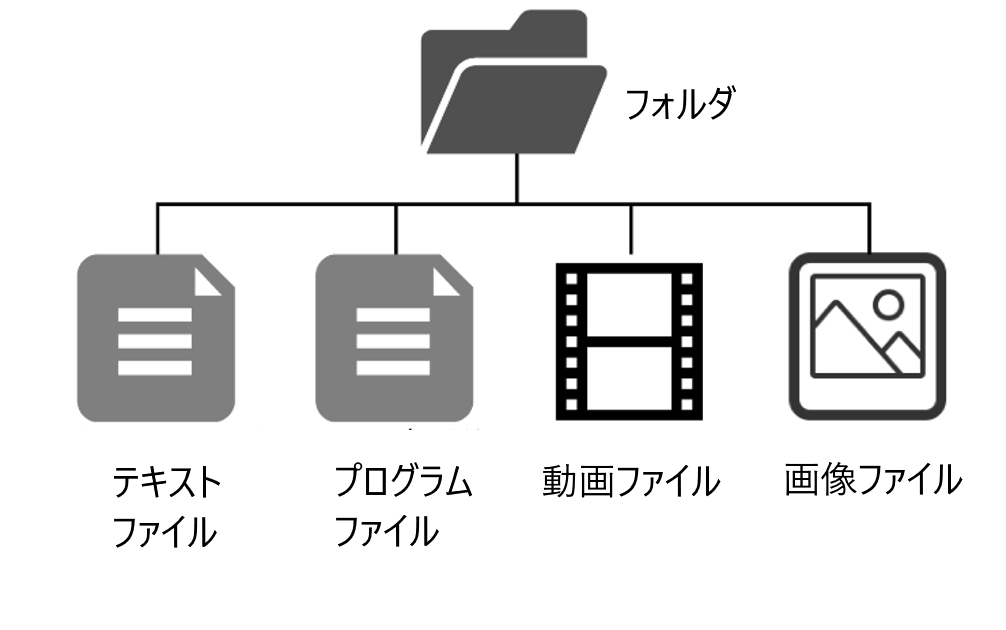
\includegraphics[width=\textwidth]{slide02_001.png}
\end{frame}

\begin{frame}[fragile]
	\frametitle{例題1-5 自分のフォルダの名前を見てみよう P.17~~~\raisebox{-3mm}{
\includegraphics[width=0.1\textwidth]{raspberry}}}
    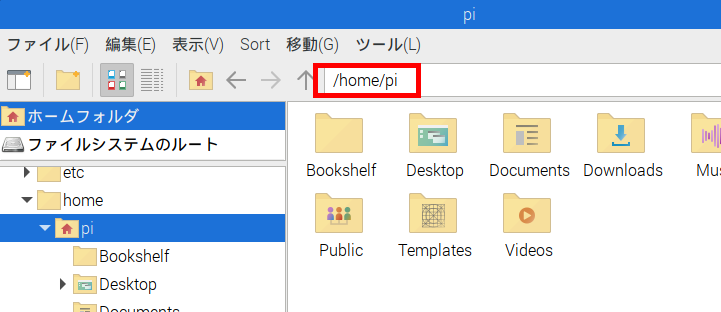
\includegraphics[width=\textwidth]{slide02_004.png}
    \vfill
    \large\textbf{教科書の17pをよんで、自分のフォルダの名前を見てみよう}
    \begin{itemize}
      \item かくにんしたら、問題1-6を問いてみよう
    \end{itemize}
\end{frame}

\begin{frame}[fragile]
	\frametitle{ファイルとフォルダのそうさになれようP.18-23~~~\raisebox{-3mm}{
\includegraphics[width=0.1\textwidth]{raspberry}}}
      \large\textbf{教科書をよみながら、じゅんばんに例題をやってみよう}
				\begin{itemize}
					\item 例題1-6 フォルダを作成しよう
					\item 例題1-7 フォルダを移動しよう
					\item 例題1-8 ファイル名を変更しよう
				\end{itemize}
      \vfill
      \large\textbf{早く終わった子は、次の問題にチャレンジしよう}
      \begin{itemize}
        \item 問題1-7, 問題1-8, 問題1-9
      \end{itemize}
      \vfill
      \large\textbf{わからないことは、放っておかず、すぐに TA に聞きましょう}
\end{frame}

\begin{frame}[fragile]
	\frametitle{キーボードの使い方をおぼえよう P.24-25~~~\raisebox{-3mm}{
\includegraphics[width=0.1\textwidth]{raspberry}}}
    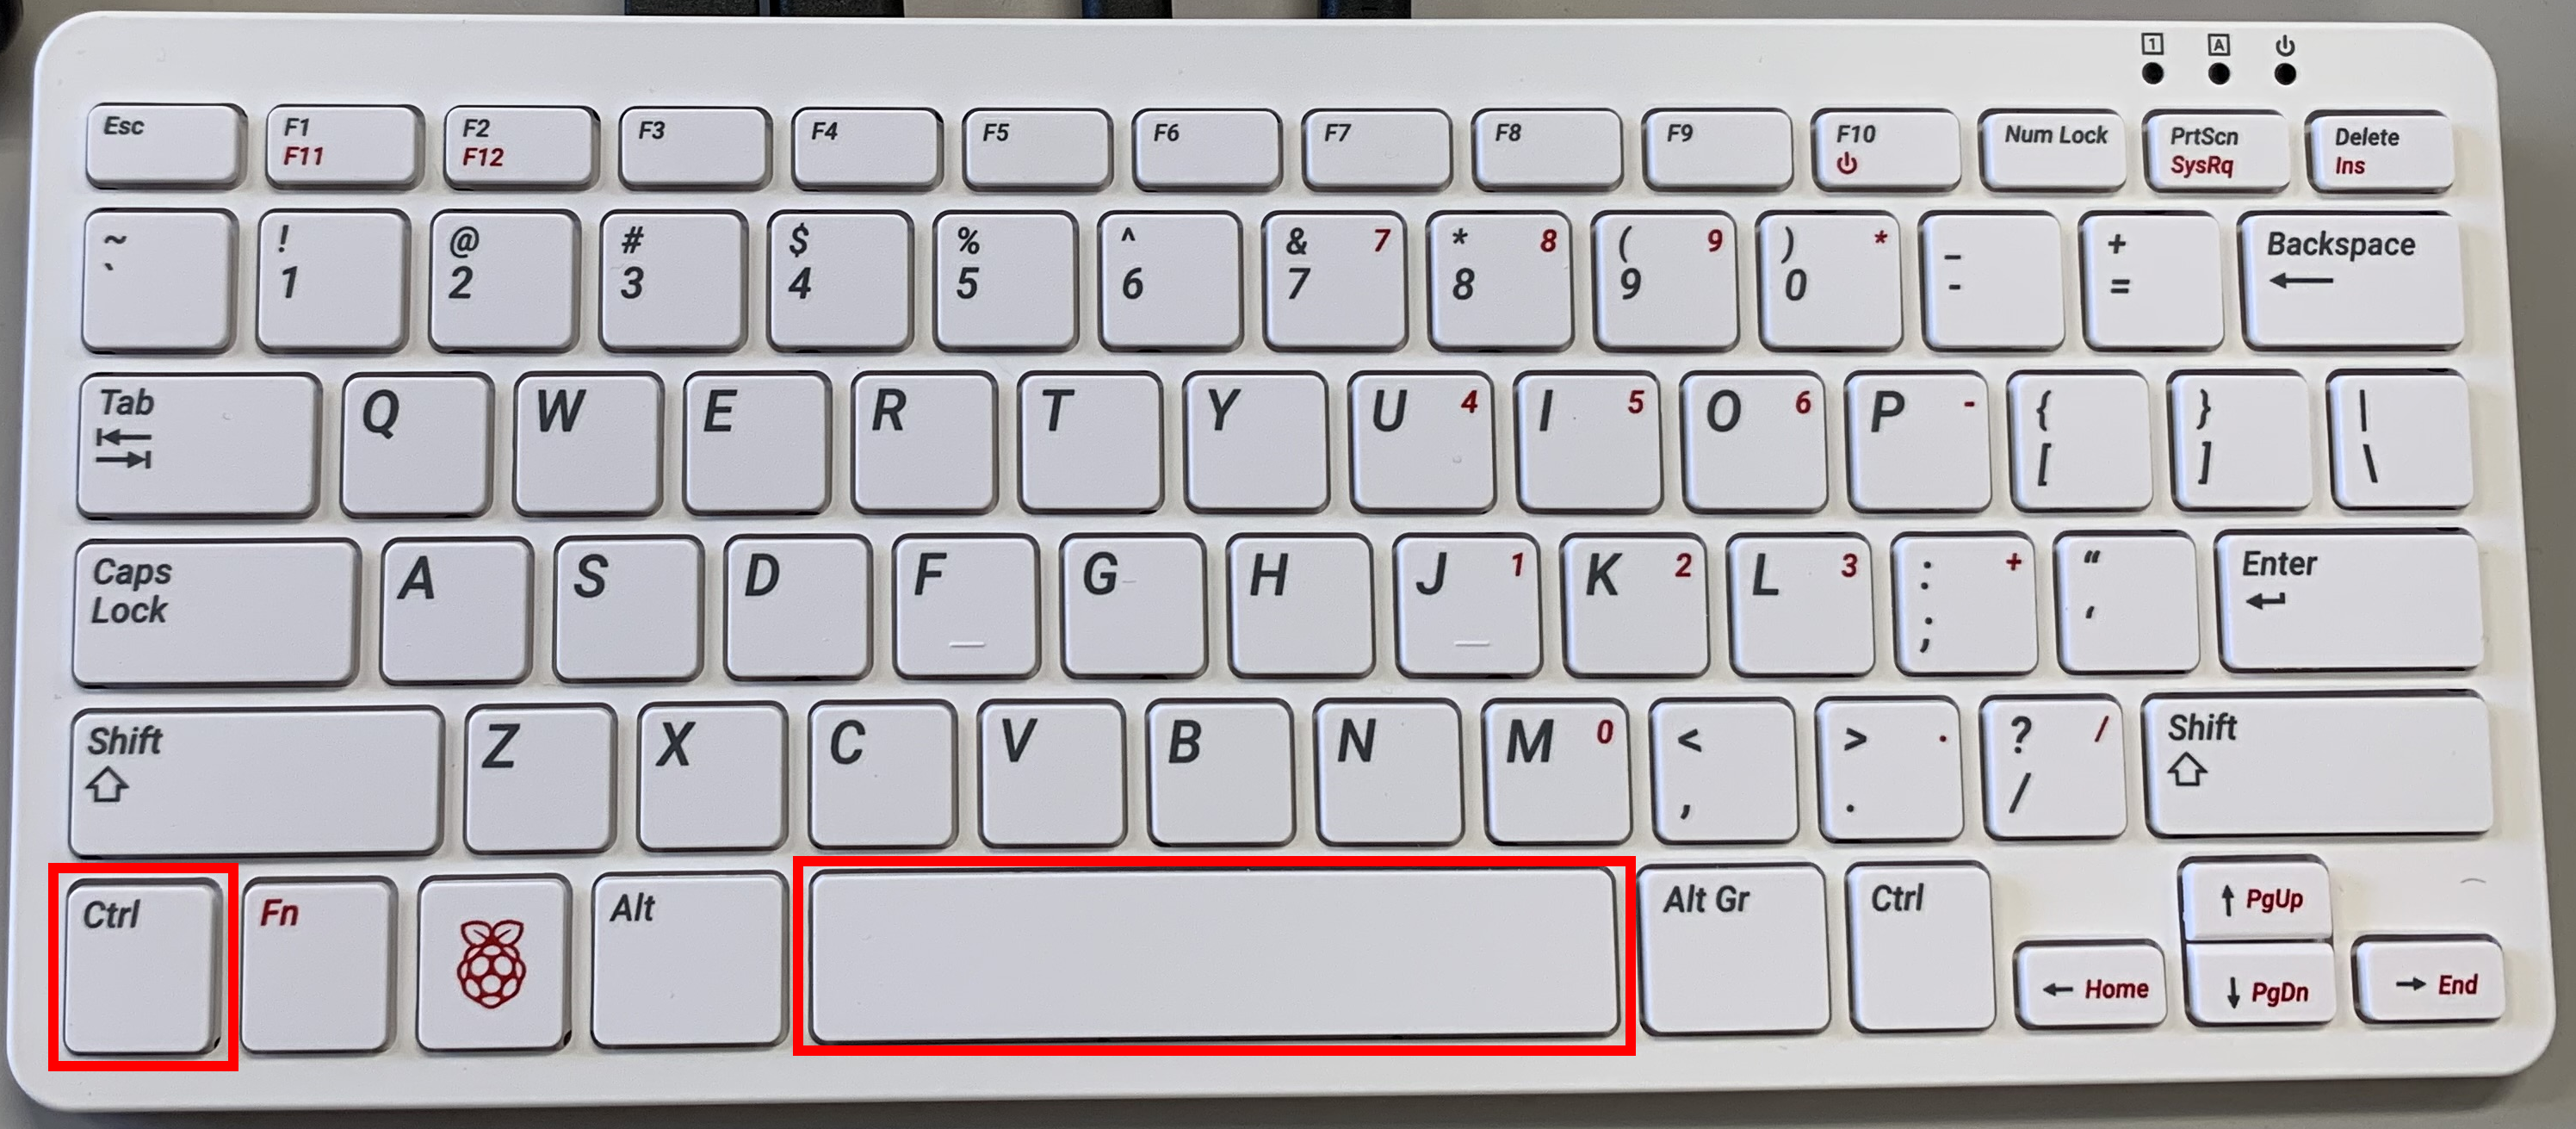
\includegraphics[width=\textwidth]{slide02_002.png}
    \vfill
    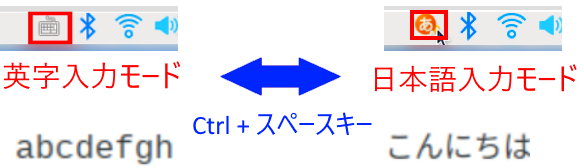
\includegraphics[width=\textwidth]{slide02_003.png}\\
\end{frame}

\begin{frame}[fragile]
	\frametitle{キーボードの使い方をおぼえよう P.24-25~~~\raisebox{-3mm}{
\includegraphics[width=0.1\textwidth]{raspberry}}}
    \large\textbf{教科書をよみながら、じゅんばんに例題をやってみよう}
    				\begin{itemize}
    					\item 例題1-9 日本語入力と英字入力について
    					\item 例題1-10 半角入力と全角入力について
    				\end{itemize}
          \vfill
          \large\textbf{早く終わった子は、次の問題にチャレンジしよう}
          \begin{itemize}
            \item 問題1-10, 問題1-11
          \end{itemize}
          \vfill
          \large\textbf{わからないことは、放っておかず、すぐに TA に聞きましょう}
\end{frame}

\begin{frame}[fragile]
	\frametitle{\large{例題1-11 ブラウザ立ち上げとマウスそうさをしようP.26-27}~~~\raisebox{-3mm}{
\includegraphics[width=0.1\textwidth]{raspberry}}}
  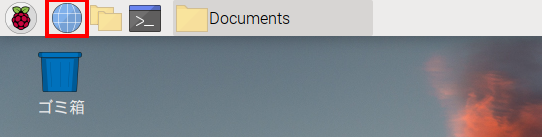
\includegraphics[width=\textwidth]{slide02_009.png}
  \vfill  
  \large\textbf{地球のアイコンを左クリックして、ブラウザを立ち上げよう}
  \vfill
  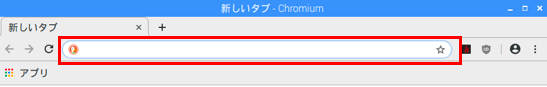
\includegraphics[width=\textwidth]{slide02_005.png}
  \vfill
  \large\textbf{赤枠の部分を左クリックして、キーボードで調べたい言葉を入力。終わったらEnterキーを押そう}\\
\end{frame}

\begin{frame}[fragile]
	\frametitle{例題1-12 キーボード入力の練習をしよう P.28-30~~~\raisebox{-3mm}{
\includegraphics[width=0.1\textwidth]{raspberry}}}
  \begin{figure}
    \centering
    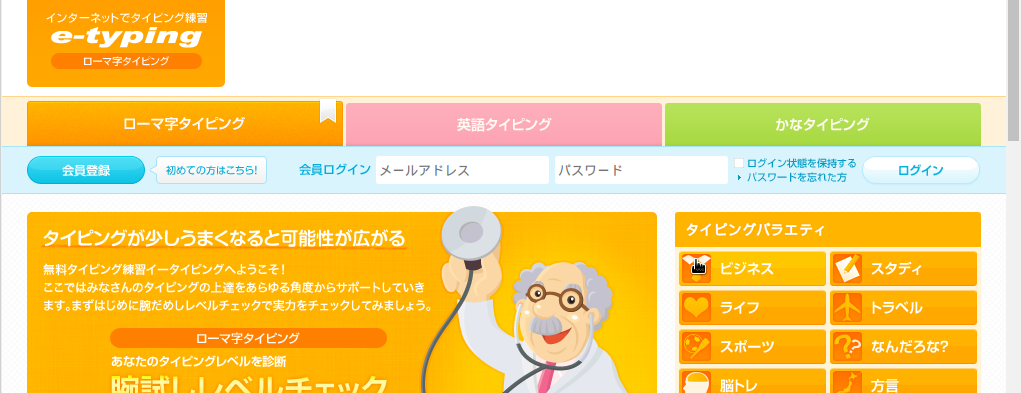
\includegraphics[width=0.7\textwidth]{slide02_010.png}
  \end{figure}
  \vfill
  \large\textbf{教科書をよみながら、タイピング練習サイトE-Typingを開こう。そして、タイピングレベルをはかってみよう}
  \begin{itemize}
    \item おわったら結果がでます。じぶんのタイピングレベルをシールカードにきろくしよう
  \end{itemize}
  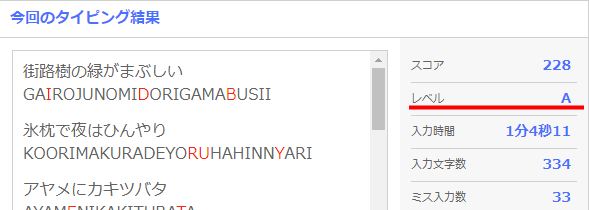
\includegraphics[width=0.62\textwidth]{slide02_012.png}
  \hfill
  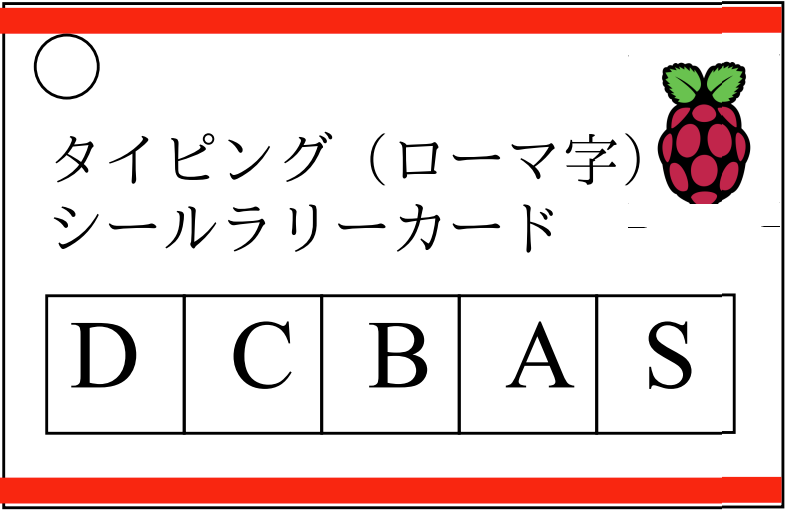
\includegraphics[width=0.34\textwidth]{slide02_011.png}
\end{frame}


\begin{frame}[fragile]
	\frametitle{ブラウザをつかってみよう P.31-33~~~\raisebox{-3mm}{
\includegraphics[width=0.1\textwidth]{raspberry}}}
    \large\textbf{教科書をよみながら、例題をやってみよう}
    				\begin{itemize}
    					\item 例題1-13 画像けんさくし、画像を保存しよう
    				\end{itemize}
          \vfill
          \large\textbf{早く終わった子は、次の問題にチャレンジしよう}
          \begin{itemize}
            \item 問題1-12, 問題1-13
          \end{itemize}
          \vfill
          \large\textbf{わからないことは、放っておかず、すぐに TA に聞きましょう}
\end{frame}

\begin{frame}[fragile]
	\frametitle{好きなように画面をへんしゅうしよう P.34-35~~~\raisebox{-3mm}{
\includegraphics[width=0.1\textwidth]{raspberry}}}
  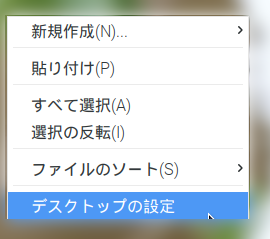
\includegraphics[width=0.35\textwidth]{slide02_007.png}
  \hfill
  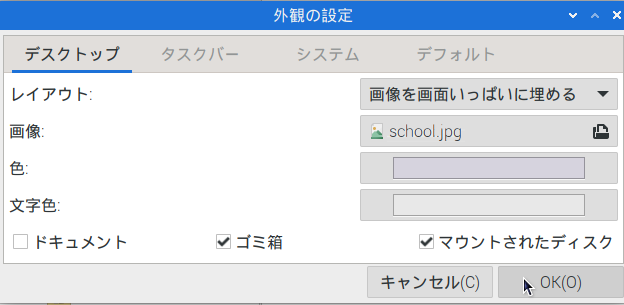
\includegraphics[width=0.62\textwidth]{slide02_008.png}
  \vfill
  \large\textbf{「デスクトップの設定」メニューをクリックすると、画面をへんしゅうすることができるよ}
  \begin{itemize}
    \item じぶんの好きなように設定しよう
  \end{itemize}

\end{frame}

\begin{frame}[fragile]
	\frametitle{好きなように画面をへんしゅうしよう P.34-35~~~\raisebox{-3mm}{
\includegraphics[width=0.1\textwidth]{raspberry}}}
    \large\textbf{教科書をよみながら、じゅんばんに例題をやってみよう}
    				\begin{itemize}
    					\item 例題1-15 ブラウザ立ち上げとマウスそうさをしよう
    					\item 例題1-16 キーボード入力の練習をしよう
    				\end{itemize}
          \vfill
          \large\textbf{同時に問題にチャレンジしよう}
          \begin{itemize}
            \item 問題1-15, 問題1-16
          \end{itemize}
          \vfill
          \large\textbf{わからないことは、放っておかず、すぐに TA に聞きましょう}
\end{frame}

\begin{frame}[fragile]
	\frametitle{\raisebox{-3mm}{
\includegraphics[width=0.1\textwidth]{raspberry}}休憩~~~\raisebox{-3mm}{
\includegraphics[width=0.1\textwidth]{raspberry}}}
	\huge
      \begin{itemize}
           \item 水分補給をしましょう
           \item 遠くのものを見て目を休めましょう
     \end{itemize}
\end{frame}

\end{document}

